\documentclass[slidestop,uncompress,mathserif,final]{beamer}
%\usecolortheme[RGB={108,0,161}]{structure}
\usecolortheme[RGB={46,1,58}]{structure}
%\usecolortheme[RGB={68,0,101}]{structure}
%\setbeamertemplate{blocks}[rounded][shadow=true] 
%\definecolor[named]{colorlightlilla}{RGB}{124,0,184} 
%\definecolor[named]{colordarklille}{RGB}{28,0,41} 
%\setbeamertemplate{background canvas}[vertical shading][bottom=colorlightlilla!20,top=colordarklille!30]
\usepackage{times}

\usepackage{color, graphicx}
\usepackage[draft]{fixme}
\usepackage[utf8]{inputenc}
\usepackage{pgf}
%\usepackage{beamerthemesplit}
\usepackage{listings}
\usepackage{tikz}
\usepackage{amsmath}
\usetikzlibrary{arrows}
%\usepackage{fancyhdr,lastpage}
%\pagestyle{fancy}\fancyhf{}\rfoot{\vspace{-0.5cm} Page
%{\thepage} of \pageref{LastPage}}
\setbeamertemplate{navigation symbols}{}    % turn off navigation symbols
%\title[Short Title \hspace{4em} \insertframenumber\ of \inserttotalframenumber]{Full Title}

%%%%%%%%%%%%%%%%%%%%%%%%%%%%%%%%%%%%%%%%%%%%%%%%%%%%%%%%%%%%%
%%% LstListing set up style for VDM
%%%%%%%%%%%%%%%%%%%%%%%%%%%%%%%%%%%%%%%%%%%%%%%%%%%%%%%%%%%%%
\lstdefinelanguage{VDM++}
  {morekeywords={act, active, fin, req, waiting, abs, all, allsuper, always, and, answer, 
     assumption, async, atomic, be, bool, by, card, cases, char, class, comp, compose, conc, cycles,
     dcl, def, definitions, del, dinter, div, dlmodule, do, dom, dunion, duration, effect, elems, else, elseif, end,
     error, errs, exists, exists1, exit, exports, ext, floor, for, forall, from, functions, 
     general, hd, if, imports, in, inds, infer, init, inmap, input, instance, int, inter, inv, inverse, iota, is, 
     isofbaseclass, isofclass, inv, inverse, lambda, len, let, map, measure, mu,
     mutex, mod, module, nat, nat1, new, merge, 
     munion, not, of, operations, or, others, per, periodic, post, power, pre, pref, 
     private, protected, public, qsync, rd, responsibility, return, reverse,  
     sameclass, parameters, psubset, rem, renamed, rng, sel, self, seq, seq1, set, skip, specified, st, 
     start, startlist, state, static, subclass, subset, subtrace, sync, system, then, thread, 
     threadid, time, tixe, tl, to, token, traces, trap, types, undefined,
     union, uselib, using, values, 
     variables, while, with, wr, yet, RESULT, false, true, nil, periodic pref, rat, real},
   %keywordsprefix=mk\_,
   %keywordsprefix=a\_,
   %keywordsprefix=t\_,
   %keywordsprefix=w\_,
   sensitive,
   morecomment=[l]--,
   morestring=[b]",
   morestring=[b]',
  }[keywords,comments,strings]
\lstdefinelanguage{JavaCC}
  {morekeywords={options, PARSER\_BEGIN, PARSER\_END, SKIP, TOKEN},
   sensitive=false,
  }[keywords]

% define the layout for listings
\lstdefinestyle{tool}{basicstyle=\ttfamily,
          frame=trBL, 
			 showstringspaces=false, 
			 frameround=ffff, 
			 framexleftmargin=0mm, 
			 framexrightmargin=0mm}
\lstdefinestyle{vdmRoundCorner}{basicstyle=\footnotesize\ttfamily,
          frame=trBL, 
          %  numbers=left, 
			 gobble=0, 
%			 basewidth=0.51em,
          showstringspaces=false, 
          captionpos=b,
			 linewidth=\textwidth, 
			 frameround=fttt, 
			 aboveskip=2mm,
			 belowskip=2mm,
			 framexleftmargin=0mm, 
			 framexrightmargin=0mm}

\lstdefinestyle{vdmNumber}{basicstyle=\footnotesize\ttfamily,
          frame=trBL, 
          numbers=left, 
			 gobble=0, 
%			 basewidth=0.51em,
          showstringspaces=false, 
          captionpos=b,
			 linewidth=\textwidth, 
			 frameround=fttt, 
			 aboveskip=2mm,
			 belowskip=2mm,
			 framexleftmargin=0mm, 
			 framexrightmargin=0mm}

\lstdefinestyle{vdmNoRoundCorner}{basicstyle=\footnotesize\ttfamily,
          frame=trBL, 
          numbers=left, 
			 gobble=0, 
%			 basewidth=0.51em,
          showstringspaces=false, 
			 linewidth=\textwidth, 
			 frameround=fttt, 
			 aboveskip=2mm,
			 belowskip=2mm,
			 framexleftmargin=0mm, 
			 framexrightmargin=0mm}
\lstdefinestyle{ast}{basicstyle=\ttfamily\small,
			 frame=tb,
%         numbers=left,
			 gobble=0,
			 showstringspaces=false,
			 linewidth=338pt,
			 frameround=ffff,
			 framexleftmargin=8mm,
			 framexrightmargin=8mm,
			 framextopmargin=1mm,
			 framexbottommargin=1mm,
			 aboveskip=7mm,
			 belowskip=5mm,
			 xleftmargin=10mm,}

\lstdefinestyle{xmlFile}{basicstyle=\footnotesize\ttfamily,
          frame=trbL, 
          numbers=left, 
			 gobble=0, 
			 basewidth=0.51em,
          showstringspaces=false, 
          captionpos=b,
			 linewidth=\textwidth, 
			 frameround=fttt, 
			 aboveskip=2mm,
			 belowskip=2mm,
			 framexleftmargin=0mm, 
			 framexrightmargin=0mm}

\lstset{style=vdmRoundCorner}
\lstset{language=VDM++}
\lstset{alsolanguage=Java}
% The command below enables you to escape into normal LaTeX mode inside your 
% VDM chunks by starting with a `!� character and ending with a `��
\lstset{escapeinside=!�}


%\lstdefinestyle{javaStyle}{basicstyle=\footnotesize\ttfamily,
%                         frame=trBL, 
%                         numbers=left, 
%			 gobble=0, 
%			 basewidth=0.51em,
%                         showstringspaces=false, 
%			 linewidth=\textwidth, 
%			 frameround=fttt, 
%			 aboveskip=2mm,
%			 belowskip=2mm,
%			 framexleftmargin=0mm, 
%			 framexrightmargin=0mm}

\usepackage{macros}
\lstdefinestyle{tool}{basicstyle=\ttfamily,
                         frame=trBL, 
			 showstringspaces=false, 
			 frameround=ffff, 
			 framexleftmargin=0mm, 
			 framexrightmargin=0mm}
\lstdefinestyle{mystyle}{basicstyle=\ttfamily,
                         frame=trBL, 
%                         numbers=left, 
%			 gobble=0, 
			 showstringspaces=false, 
%			 linewidth=\textwidth, 
			 frameround=fttt, 
			 aboveskip=5mm,
			 belowskip=5mm,
			 framexleftmargin=0mm, 
			 framexrightmargin=0mm}
%\lstdefinestyle{mystyle}{basicstyle=\sffamily\small,
%			 frame=tb,
%                         numbers=left,
%			 gobble=0,
%			 showstringspaces=false,
%			 linewidth=345pt,
%			 frameround=ffff,
%			 framexleftmargin=8mm,
%			 framexrightmargin=8mm,
%			 framextopmargin=1mm,
%			 framexbottommargin=1mm,
%			 aboveskip=7mm,
%			 belowskip=5mm,
%			 xleftmargin=10mm,}

\lstset{style=mystyle}
\lstset{language=VDM++}
\lstset{alsolanguage=Java}
% The command below enables you to escape into normal LaTeX mode inside your 
% VDM chunks by starting with a `?´ character and ending with a `£´
%\lstset{escapeinside=?£}

%\usetheme{Singapore} 
\usetheme{Copenhagen} 

% Util commands %
\newcommand{\pgl}[0]{Peter Gorm Larsen} 
\newcommand{\mail}[1]{{\small \texttt{#1}}}
\newcommand{\yellow}[1]{{\color{yellow} #1}}
\newcommand{\blue}[1]{{\color{blue} #1}}
\newcommand{\red}[1]{{\color{red} #1}}
\newcommand{\green}[1]{{\color{green} #1}}
\newcommand{\fixin}[1]{\fixme[inline]{\texttt{#1}}} 
\newcommand{\fixfo}[1]{\fixme[footnote]{\texttt{#1}}} 
\newcommand{\fixma}[1]{\fixme[margin]{\texttt{#1}}} 
\newcommand{\from}[1]{%
\noindent%
\begin{flushright}%
    \emph{\footnotesize #1}%
\end{flushright}%
} 
%\usebackgroundtemplate{\includegraphics[width=\paperwidth]{images/bg.png}}
\title{Connecting UML and VDM++ with Open Tool Support}

\subtitle{16th International Symposium on Formal Methods}

\author[K. Lausdahl, H.K.A Lintrup, P.G. Larsen]{
  Kenneth Lausdahl \\
  \mail{kenneth@lausdahl.com} \\
  Hans Kristian Agerlund Lintrup \\
  \mail{hlintrup@gmail.com}\\
  Peter Gorm Larsen \\
  \mail{pgl@iha.dk}
}

\institute[IHA]{
  Aarhus School of Engineering
}

%\pgfputat{\pgfxy(0,-6.5)}{\pgfbox[left,base]{
\includegraphics[width=2cm]{images/OMLlogoattempt.jpg}}}

\date{Eindhoven --- November 2009}

\begin{document}

%
% Table of conent frame
%
\begin{frame}[c]
	\titlepage
\end{frame}

\begin{frame}[c]
  \frametitle{Outline}
  \tableofcontents %[pausesections] %[current,currentsubsection]
%  \tableofcontents[current]
\end{frame}


%#######################################################################
%
% Introduction and motivation for open tool support and VDM + UML
%
\section{Introduction}
%-----------------------------------------------------------------------

%-----------------------------------------------------------------------
\subsection{Background}
%-----------------------------------------------------------------------

%
% Motivation
%
\frame
{
 \frametitle{Motivation}
%\begin{center}
  \begin{itemize}[<+->]
\itemsep=1cm
  \item<1-> Best of both by combining VDM and UML.
  \item<2-> Improve the tool support for VDM.
%  \item<3-> Provide an easy to use and extensible user interface.
  \end{itemize}
%\end{center}
}
\note{
VDM = precession
UML = overview, less details

}
%
% Motivation combining knowlage
%
%\frame
%{
%\frametitle{Communication}
%  \begin{itemize}
%	\itemsep=1cm
%  		\item<1-> Formal Method (VDM)
%  		\item<2-> Unified Modeling Language (UML)
%  		\item<3-> Provide a broader platform of information sharing
%  \end{itemize}
%
%}

\note
{

  \begin{itemize}
	%\itemsep=1cm
  		\item Use a formal method to exactly specify what the system should do and prove that it does so.
  		\item Use UML to communicate to domain experts, thus a larger number of people can verify the model.
  		
  \end{itemize}



}

%
% Goal
%
\frame
{
  \frametitle{Goal}

\begin{center}

	\begin{block}<+->{Transformation}
	Provide a bidirectional connection between VDM and UML 2.1.2. 
	\begin{itemize}
		\item Class Diagrams
		\item Sequence Diagrams (new)
	\end{itemize}
	\end{block}
\vspace{1cm}
	\begin{block}<+->{Tool}
	Provide a open source tool as part of the Overture Tool suite
	\end{block}
%  \begin{itemize}
%	%\itemsep=1cm
%  		\item Provide a connection between VDM and UML
%  		\item Display a VDM static structure diagram (Class Diagram)
%  		\item Creation of Combinatorial Test statements from a dynamic diagram (Sequence Diagram)
%  		\item Integrate the transformation tool into Eclipse
%  		\item Open source
%	  	
%  \end{itemize}
\end{center}
}


%-----------------------------------------------------------------------
\subsection{Vienna Development Method}
%-----------------------------------------------------------------------
%
% VDM
%
\frame
{
  \frametitle{The Vienna Development Method}


  \begin{itemize}
	%\itemsep=1cm
  		\item<1-> VDM originates from Vienna in the 1970s
  		\item<1-> VDM Specification Language (VDM-SL) ISO standardised in '96
  		\item<2-> Extended in 1992-94 with object oriented structure and concurrency handling (VDM++).
  		\item<3-> Extended in 1999-2007 with distributed real-time systems (VICE).
	  	\item<4-> VDM++ Extended with Traces for test automation in 2008
  		\item<5-> Two most significant tool suites.
  		\begin{itemize}
  			\item<6-> VDM Tools - commercial
			\begin{itemize}
				\item Existing bidirectional link to UML 1.4.2 (Rational Rose)
				\item First released in 1997
			\end{itemize}
  			\item<7-> Overture - open source
			\begin{itemize}
				\item New bidirectional link to UML 2.1.2 (Enterprise Architect)
				\item First released in 2009
			\end{itemize}
  		\end{itemize}

  \end{itemize}


}

%
% Small VDM example
%
\frame
{
  \frametitle{VDM Train example}

\begin{center}

\vdmSpecLineNum{ClassDiagramOverview.vpp}{VDM classes with collections.}{VDM:Collections}

\end{center}
}

%-----------------------------------------------------------------------
\subsection{Unified Modeling Language}
%-----------------------------------------------------------------------
%
% UML
%
\frame
{
  \frametitle{Unified Modeling Language - UML}

	\begin{itemize}
	%\itemsep=1cm
  		\item<1-> UML is a semi-formal visual modeling language
		\item UML 1.4.2 - ISO 2005
		\item UML 2.1.2 - 2007 
  		\item<2-> Enabled developers to look at the system from different view points.
  		\item<3-> Comprised of different kinds of diagrams.
		\begin{itemize}
			%\item Primiary categoies of diagrams
			%\begin{itemize}
				\item Structure: Class Diagrams
				\item Behavior: Sequence Diagrams (significant improvements in UML 2.1.2)
			%\end{itemize}
		\end{itemize}
  		 
	  	
  \end{itemize}

}

\note
{
Used by developers to model a system at a desired level of abstraction.

Sequence diagrams: loops, alt

}


%
% Class Diagram
%
\frame
{
  \frametitle{Class Diagram}

\begin{center}

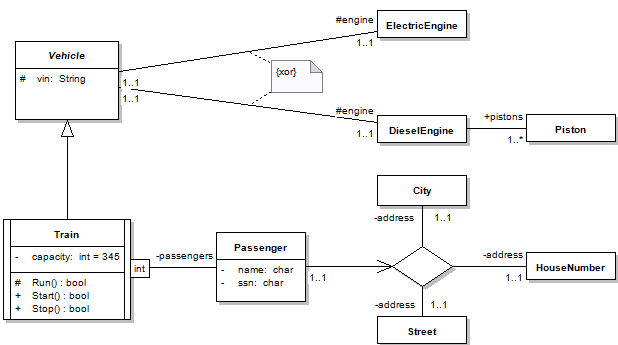
\includegraphics[width=\textwidth]{images/ClassDiagramOverview.png}

\end{center}
}

\note
{
\begin{itemize}
	\item Active class
	\item Generalization
	\item Visibility: public, proteted, private
	\item Association
	\begin{itemize}
		\item Qualified (int)
		\item N-ary
		\item Constraint (xor)
	\end{itemize}
\end{itemize}

}

%
% Sequence Diagram
%
\frame
{
  \frametitle{Sequence Diagram}

\begin{center}
	\includegraphics<1->[width=0.5\textwidth]{images/SequenceDiagram.png}%
\end{center}
}


\note
{
\begin{itemize}
	\item Life line
	\item Alternative: alt
	\item Loop
	\item Constraint
\end{itemize}

}



%#######################################################################
%
% Introduction and motivation for open tool support and VDM + UML
%
\section{Connecting UML and VDM++}
%-----------------------------------------------------------------------
%
% Outline
%
\begin{frame}
  \frametitle{Outline}
  \tableofcontents[current]
\end{frame}


%-----------------------------------------------------------------------
%\subsection{History}
%-----------------------------------------------------------------------
%
% VDM Tools
%
%\frame
%{
%  \frametitle{Existing tool}
%
%VDM Tools
%  \begin{itemize}
%	%\itemsep=1cm
%  		\item<1-> Commercial tool from CSK
%  		\item<2-> No editor
%  		\item<3-> Includes a UML transformation
%  		\begin{itemize}
%  			\item Rose VDM Link first release (1997)
%  			\item UML 1.4
%  		\end{itemize}
%	  	
%  \end{itemize}
%
%
%}
%
%
%\note
%{
%
%  \begin{itemize}
%	%\itemsep=1cm
%  		\item Only tool
%  		\item Commercial
%  		\item Older UML Transformation Rose VDM Link from (1997)
%  		\item UML 1.4
%	  	
%  \end{itemize}
%
%
%
%
%}


%-----------------------------------------------------------------------
\subsection{Using Sequence diagrams for test automation}
%-----------------------------------------------------------------------

%
% extending uml trans
%
%\frame
%{
%  \frametitle{Extending UML support}
%
%  \begin{itemize}
%	\itemsep=1cm
%  		\item<1-> Change to UML version 2.x
%  		\item<2-> Extend UML subset for Class Diagrams
%  		\item<3-> UML Sequence Diagrams
%	  	
%  \end{itemize}
%
%
%}
%
%\note
%{
%
%  \begin{itemize}
%	%\itemsep=1cm
%  		\item Since UML 2 has since been released look into new features and uses
%  		\item Extending the subset of UML used to model VDM, active, abstract,x-or association
%  		\item Look into new diagrams which could be use full, new VDM feature for testing \textbf{Traces}
%	  	
%  \end{itemize}
%
%}


%
% Traces
%
%\frame
%{
%  \frametitle{Combinatorial Testing in VDM}
%
%  \begin{itemize}
%	%\itemsep=1cm
%  		\item<1-> New feature recently introduced to VDM - 2008
%  		\item<2-> Automatic execution of a large number of test cases generated from templates in form of trace definitions
%  		\item<3-> Add graphical representation of trace definitions in UML as Sequence Diagrams
%	  	
%  \end{itemize}
%
%
%}

%
% Traces example
%
%\frame
%{
%  \frametitle{VDM Combinatorial Test example}
%\begin{center}
%\vdmSpecLineNum{UseStack.vpp}{Traces}{VDM:Collections}
%
%\end{center}
%}



%
% Traces example expanded
%
\begin{frame}[fragile] 

  \frametitle{VDM Combinatorial Test example evaluation}
\begin{columns}
\begin{column}[l]{5cm}

%\begin{itemize}\footnotesize
%\item Set selection \tikz\node [fill=blue!20,draw,circle] (n1) {};
%\item Repeat \tikz\node [fill=red!20,draw,circle] (n2) {};
%\end{itemize}

	\begin{center}
\onslide<2->{ 
\begin{tikzpicture}
[
	overlay,
	xscale	= 1,	% to scale horizontally everything but the text
	yscale	= 1,	% to scale vertically everything but the text
]
	\node[fill=blue!20,text height=0.2ex,text width=2ex, text depth=0.25ex]	at	(1.3,-1.7) (t1){ };

	\node[fill=red!20,text height=0.2ex,text width=2ex, text depth=0.25ex]	at	(1.9,-2.5) (t1){ };

	\node[fill=green!20,text height=0.2ex,text width=0.5ex, text depth=0.25ex]	at	(-0.6,-3.7) (t1){ };
\end{tikzpicture}
}
	\vdmSpecLineNum{UseStackTrace.vpp}{Traces}{VDM:Collections}
	\end{center}

\end{column}
\begin{column}[r]{5cm}
	\begin{itemize}
		\item<3-> TC1:
		\begin{itemize}
			\item stack.Reset()
			\item stack.Push(2)
			\item stack.Push(5)
		\end{itemize}
		\item<4-> TC2:
		\begin{itemize}
			\item stack.Reset()
			\item stack.Push(8)
			\item stack.Push(8)
			\item stack.Pop()
		\end{itemize}
		\item<5-> ... 14 more
	\end{itemize}



\end{column}
\end{columns}
\end{frame}
\note{
show x in set (2,8)
show {1,4} repeat
show choice |

}


\frame
{
  \frametitle{Combinatorial Test form Overture}
	\begin{center}
	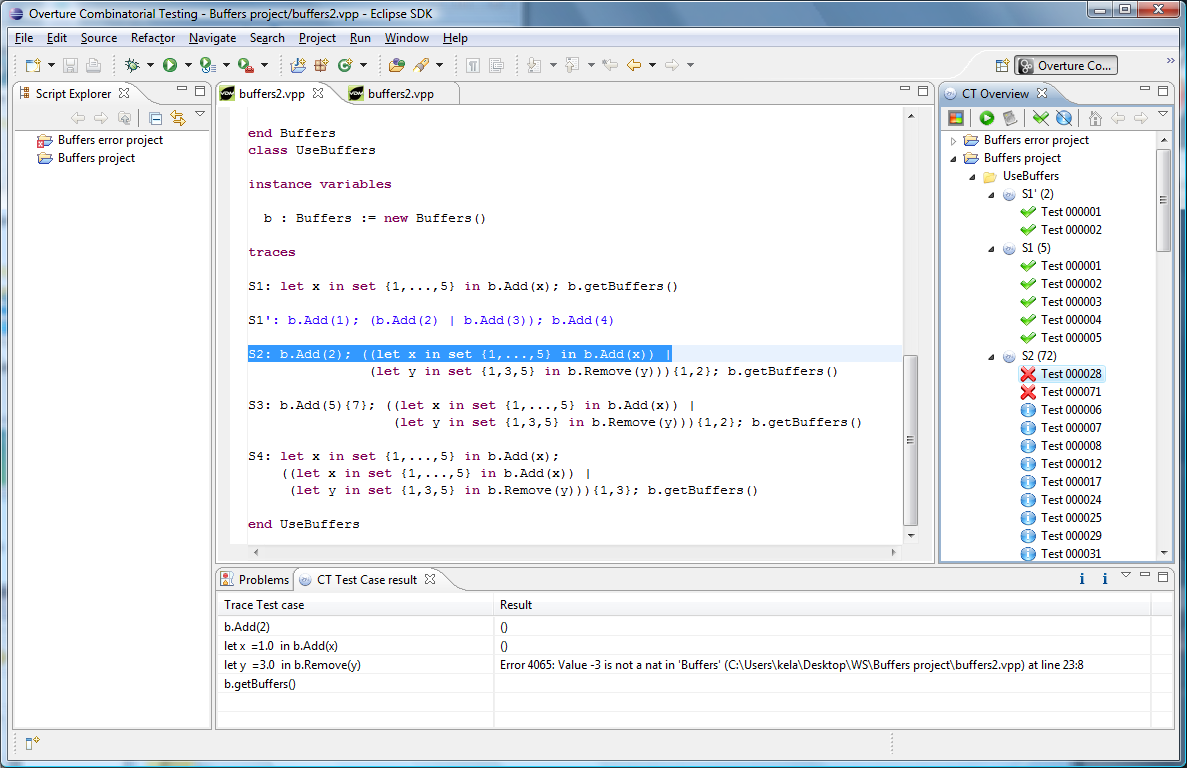
\includegraphics[width=0.85\textwidth]{images/CTOverview.png}%
	\end{center}
}

%
% Traces example UML
%
\frame
{
  \frametitle{VDM Combinatorial Test example Sequence Diagram}
  
\begin{columns}
\begin{column}[l]{5cm}

	\begin{center}
	\vdmSpecLineNum{UseStackTrace.vpp}{Traces}{VDM:Collections}
	\end{center}

\end{column}
\begin{column}[r]{5cm}
	
	\begin{center}
	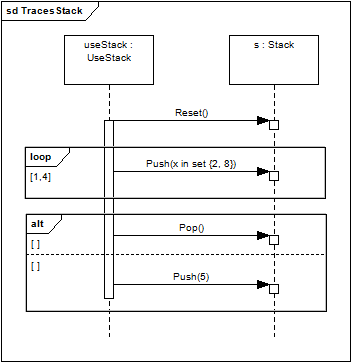
\includegraphics[width=\textwidth]{images/TracesSequenceDiagramEx2.png}%
	\end{center}

\end{column}
\end{columns}
  

}




%#######################################################################
%
% Introduction and motivation for open tool support and VDM + UML
%
\section{Tool building in VDM}
%-----------------------------------------------------------------------
%
% Outline
%
\begin{frame}
  \frametitle{Outline}
  \tableofcontents[current]
\end{frame}



%
% Improce Tools support
%
\frame
{
  \frametitle{Tool building in VDM}
\begin{center}
  \begin{itemize}
	%\itemsep=1cm
  		\item AST creation in VDM-SL
  		\item VDM for molding of AST
  		\item VDM Tools code generator to Java
  		\item Eclipse plug-in building.
	  	
  \end{itemize}

\end{center}
}







%-----------------------------------------------------------------------
\subsection{AST modeling}
%-----------------------------------------------------------------------

%
% UML Transformation overview
%
\frame
{
  \frametitle{AST creation}

\begin{center}
\begin{figure}
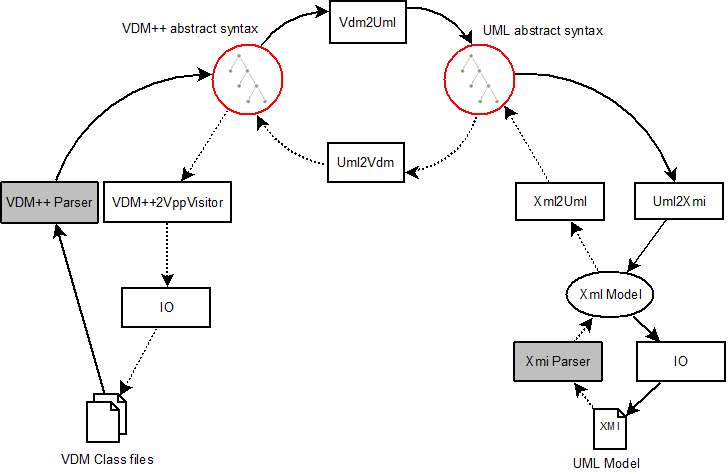
\includegraphics[width=\textwidth]{images/OverviewOverMappingAST.png}
\end{figure}
\end{center}
}


%
% Overview of supported features
%
\frame
{
  \frametitle{Creating AST's from VDM-SL}
\begin{center}



\begin{columns}
\begin{column}[l]{4cm}

  \begin{itemize}
	%\itemsep=1cm
  		\item Create VDM-SL tree
  		\item ASTGen to VDM and Java
  		\item Model in VDM
  		\item VDM Tools code generator to Java
  \end{itemize}

\end{column}
\begin{column}[r]{6cm}

\vdmSpecLineNum{UMLAST_Class.ast}{}{VDM:Collections}


\end{column}
\end{columns}


\end{center}
}


%-----------------------------------------------------------------------
\subsection{Transformation modeling}
%-----------------------------------------------------------------------

%
% Overview Modeling
%
\frame
{
  \frametitle{VDM model}
\begin{center}


\vdmSpecLineNum{Vdm2UmlBuild_class.vpp}{}{VDM:Collections}



\end{center}
}

%-----------------------------------------------------------------------
\subsection{Code generating}
%-----------------------------------------------------------------------


%
% UML Transformation overview
%
\frame
{
  \frametitle{Code generation overview}

\begin{center}

\begin{figure}

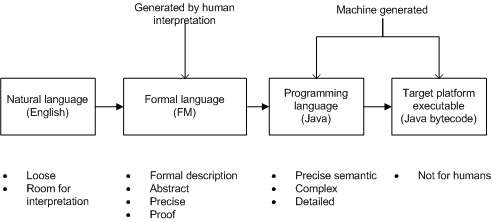
\includegraphics[width=\textwidth]{images/codegenneration.png}

\end{figure}

\end{center}
}




\begin{frame}[plain,c]
  \begin{center}
	\LARGE \structure{Thank you!}

	\vspace{2cm}
	\href{www.overturetool.org}{www.overturetool.org}
\end{center}
\end{frame}



\bibliographystyle{plain}
\bibliography{mf}



\end{document}
